\documentclass[11pt,letterpaper]{article}
\usepackage[margin=0.85in]{geometry}
\usepackage[T1]{fontenc}
\usepackage[utf8]{inputenc}
\usepackage{lmodern}
\usepackage{microtype}
\DisableLigatures{encoding=T1,family=lmtt}
\usepackage{amsmath,amssymb}
\usepackage{booktabs,tabularx,array}
\usepackage{xcolor}
\usepackage{tikz}
\usetikzlibrary{arrows.meta,positioning}
\usepackage{listings}
\usepackage{enumitem}
\usepackage{fancyhdr}
\usepackage{hyperref}
\definecolor{navy}{HTML}{173553}
\definecolor{teal}{HTML}{167D8D}
\definecolor{pale}{HTML}{F1F6FA}
\hypersetup{colorlinks=true,linkcolor=navy,urlcolor=teal,citecolor=teal,
  pdftitle={QubitSky: Classical Baselines for Acoustic Drone Detection},
  pdfauthor={QubitSky Project}}
\lstset{basicstyle=\ttfamily\footnotesize,breaklines=true,columns=fullflexible,
  keepspaces=true,showstringspaces=false,backgroundcolor=\color{pale},
  frame=single,rulecolor=\color{navy!20},xleftmargin=4pt,xrightmargin=4pt}
\setlist{itemsep=2pt,topsep=4pt}
\setlength{\parskip}{4pt}
\setlength{\parindent}{0pt}
\setlength{\headheight}{14pt}
\pagestyle{fancy}
\fancyhf{}
\lhead{\small\textcolor{navy}{QubitSky | Classical Methods}}
\rhead{\small Models A--D}
\cfoot{\small\thepage}
\newcolumntype{Y}{>{\raggedright\arraybackslash}X}
\newcommand{\code}[1]{\texttt{\detokenize{#1}}}
\newcommand{\R}{\mathbb{R}}
\title{\textcolor{navy}{\textbf{QubitSky}}\\[6pt]
  Classical Baselines for Acoustic Drone Detection\\[5pt]
  \large Models A--D, Evaluation Protocol, and CPU/CUDA Execution}
\author{QubitSky Project}
\date{October 7, 2026}

\begin{document}
\maketitle
\thispagestyle{fancy}

\begin{abstract}
This report describes four classical baselines for distinguishing drone audio
from background and acoustically similar confusers. Models A, B, and C use a
shared compact feature representation with an RBF support vector machine, a
small multilayer perceptron, and a larger multilayer perceptron, respectively.
Model D uses a convolutional neural network operating on log-mel spectrograms.
The protocol separates source recordings before windowing, fits preprocessing
on training data, selects configurations on validation data, and evaluates noise
robustness using controlled signal-to-noise ratios. Automatic CUDA detection
allows Model D to use a compatible visible GPU or fall back to CPU.
This is a methods document: it reports no new trained-model accuracy, runtime
benchmark, or evidence of quantum advantage.
\end{abstract}

\section{Purpose and implementation scope}
The binary label is $y=1$ for drone and $y=0$ for non-drone. The objective is to
establish reproducible classical reference points across model capacity and
audio noise conditions. The models serve complementary roles:

\begin{center}
\small
\begin{tabularx}{\linewidth}{@{}lYY@{}}
\toprule
Model & Input and classifier & Role in the comparison \\
\midrule
A & Compact MFCC/PCA features; RBF SVM & Nonlinear kernel baseline \\
B & Same compact features; one small hidden layer & Limited-capacity neural baseline \\
C & Same compact features; two larger hidden layers & Higher-capacity tabular baseline \\
D & Log-mel spectrogram; three convolution layers & Reference using richer temporal information \\
\bottomrule
\end{tabularx}
\end{center}

Neither C nor D is guaranteed to achieve the best accuracy. Likewise, B is not
claimed to match a quantum model's parameter budget without an explicit count
and agreed definition of capacity.

\textbf{Snapshot boundary.} The baseline described here follows the reviewed
\code{qsky_classical/cli.py}, \code{data.py}, \code{models.py}, and \code{cnn.py}
snapshot captured on October 7, 2026 at 20:23 UTC. File fingerprints accompany
this document in \code{classical_approach_sources.json}. Protocol-import,
recording-aggregation, and subset utilities were being developed concurrently;
their presence is not treated as proof of an integrated, validated experiment.
Section~\ref{sec:matched} distinguishes the comparison requirements from the
baseline CLI behavior documented here.

\clearpage
\section{Datasets and source attribution}
\label{sec:datasets}
The intended data sources follow \code{QubitSky_DATASETS.md},
\code{DATASET_SETUP.md}, and the repository's downloader. Table~\ref{tab:datasets}
states their project roles; it does not assert that every dataset has been
downloaded or used in a completed run. Actual membership, class counts, and
exclusions must come from the run's manifests and inventories.

\begin{table}[htbp]
\centering
\small
\begin{tabularx}{\linewidth}{@{}>{\raggedright\arraybackslash}p{3.5cm}YY@{}}
\toprule
Dataset & Published resource & Intended QubitSky role \\
\midrule
DDL~\cite{ddl} & Field and synthesized drone audio; the downloader selects
the real-recording archive & Main drone source; verify available labels before
constructing the binary task \\
ESC-50~\cite{esc50} & 2,000 five-second clips across 50 environmental classes
& Selected non-drone confusers and a separately reserved noise pool \\
UrbanSound8K~\cite{urbansound} & 8,732 urban-sound excerpts of at most four
seconds across 10 classes & Selected urban/mechanical confusers and additive noise \\
NASA Small UAS~\cite{nasa} & Small unmanned-aircraft flyover acoustic recordings
& External evaluation only; never training, validation, or preprocessing fitting \\
\bottomrule
\end{tabularx}
\caption{Primary dataset sources and intended roles. Published corpus sizes
are not the effective training-set sizes after filtering and grouping.}
\label{tab:datasets}
\end{table}

\paragraph{DDL: field recordings.}
Safavi et al.'s release provides separate real and synthesized
archives~\cite{ddl}. The project selects \code{MLSP_2022_Real_Data.zip}.
The publisher documents \code{MINI} and \code{PRO4} as drone classes and
\code{XXXX} as no drone, together with flight/session and sequence identifiers.
Consecutive fragments must be reconstructed in sequence within their source
session before windowing; they must not be randomly split as independent
recordings. The repository's setup notes report no \code{XXXX} examples in the
inspected real archive. Therefore, the naming convention alone does not establish
that the selected archive supplies negative examples.

\paragraph{ESC-50 and UrbanSound8K: confusers and noise.}
The ESC-50 selection contains helicopter, airplane, wind, rain, thunderstorm,
chirping birds, crow, crickets, insects, siren, footsteps, and fireworks.
These 12 classes correspond to 480 published clips before any additional
filtering~\cite{esc50}. UrbanSound8K contributes the selected classes engine
idling, siren, car horn, gun shot, street music, drilling, and
jackhammer~\cite{urbansound}. These are project-specific binary selections,
not the original 50-class or 10-class benchmark tasks.

Preserve ESC-50's \code{src_file}, UrbanSound8K's \code{fsID}, and the
published fold metadata~\cite{esc50,urbansound}. Both corpora derive from
Freesound: if the same source ID occurs in both, keep its excerpts in one split.
Assign distinct source recordings to labeled confusers and additive-noise pools.
Comparisons to published UrbanSound8K classification benchmarks require its
prescribed ten-fold evaluation; this project-specific binary protocol is not
that benchmark~\cite{urbansound}.

\paragraph{NASA: external transfer evaluation.}
The NASA portal provides the flyover archive and its data-description
document~\cite{nasa}. The repository setup notes describe MATLAB recordings
requiring conversion before waveform ingestion. Preserve acquisition metadata
and keep all derived files external-only. Establish valid labels before reporting
accuracy or F1. If labels are unavailable, report prediction summaries rather
than external classification accuracy.

\subsection{Additional sources in the teammate protocol}
The previously reviewed teammate branch also references Fredrik Svanstr\"om's
drone-detection dataset~\cite{svanstrom} and the ITU ARIS Lab.
Acoustic Drone Dataset~\cite{ituaris}. These are distinct resources from the
DDL real archive above. The ITU release contains overlapping one-second
segments and source-interval mappings; its provided group assignments must be
preserved rather than randomly splitting adjacent files. Reproducing the
teammate's experiment requires the exact dataset versions and source IDs in her
manifests, not substitution based on a shared folder name such as \code{ddl}.

Dataset links and bibliographic details below were checked on October 7, 2026.
Retain the source metadata and per-recording attribution with each downloaded
release.

\section{Data organization and audio preparation}
\subsection{Recording manifests and leakage prevention}
A signal CSV provides \code{path}, \code{label}, and optionally \code{group_id}
and \code{split}. Related excerpts from one recording, flight, or session must
share a group identifier. Paths are resolved relative to the manifest, unless
absolute. A separate noise manifest supplies additive-background recordings.

The default automatic split is approximately 60\% training, 20\% validation,
and 20\% test \emph{by source groups}; it is stratified by group label. Unequal
group sizes can produce different proportions of files or windows. Explicit
splits must cover every row, keep groups disjoint, and contain both labels in
each signal split. Mixed-label groups require explicit assignments. The data
reader also recognizes \code{validation} and \code{valid} as \code{val}.

Splitting occurs before audio is expanded into windows. The baseline runner
rejects shared file paths or source-group identifiers between the signal and
noise manifests. Training augmentation uses only training noise, and test
corruption uses only test noise. External NASA data, if used, must remain
outside training and validation; the generic CSV interface relies on the
manifest preparer to enforce that dataset role.

\subsection{Waveform preparation}
Each recording is converted to mono and resampled to $f_s=16{,}000$ Hz. The
reviewed baseline CLI uses non-overlapping one-second windows, each containing
$N=16{,}000$ samples. The final incomplete window is zero-padded rather than
discarded. Each window $x$ is peak-normalized:
\begin{equation}
 \widetilde{x}[n]=\frac{x[n]}{\max\!\left(\max_m |x[m]|,10^{-12}\right)}.
\end{equation}
This removes absolute amplitude as a direct cue. A short padded tail still
contributes a full window, so its influence should be considered during
recording-level aggregation. The current data helpers accept other durations;
the reviewed CLI still invokes their one-second default.

\begin{figure}[htbp]
\centering
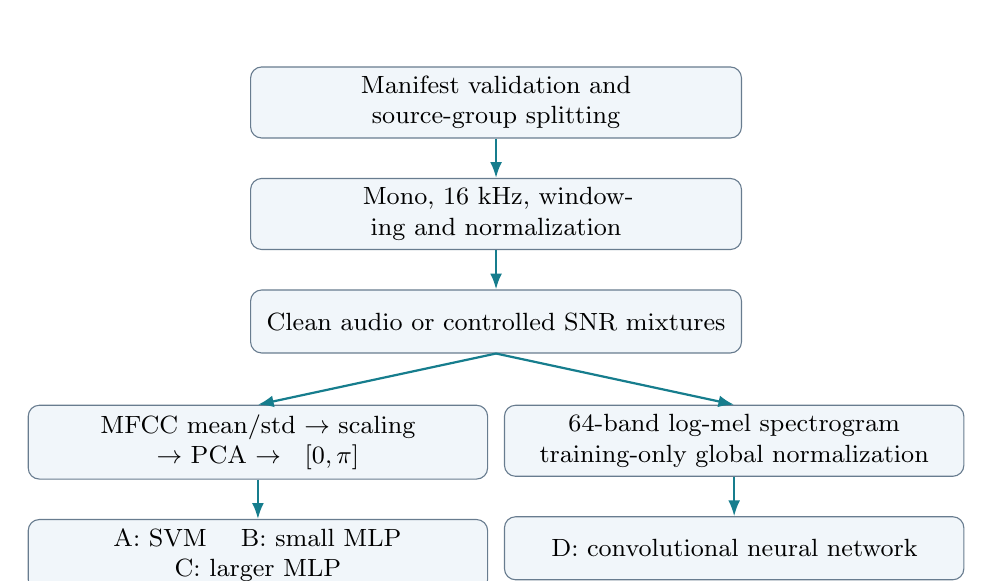
\begin{tikzpicture}[
  box/.style={draw=navy!65,rounded corners,fill=pale,align=center,
    font=\small,text width=6.0cm,minimum height=0.8cm},
  branch/.style={box,text width=5.6cm},
  flow/.style={-{Latex[length=2mm]},thick,draw=teal},node distance=0.5cm]
 \node[box] (split) {Manifest validation and source-group splitting};
 \node[box,below=of split] (audio) {Mono, 16 kHz, windowing and normalization};
 \node[box,below=of audio] (noise) {Clean audio or controlled SNR mixtures};
 \node[branch,below left=0.65cm and 0.1cm of noise.south] (tab)
   {MFCC mean/std $\rightarrow$ scaling\\$\rightarrow$ PCA $\rightarrow [0,\pi]$};
 \node[branch,below right=0.65cm and 0.1cm of noise.south] (mel)
   {64-band log-mel spectrogram\\training-only global normalization};
 \node[branch,below=of tab] (abc) {A: SVM \quad B: small MLP\\C: larger MLP};
 \node[branch,below=of mel] (cnn) {D: convolutional neural network};
 \draw[flow] (split)--(audio);
 \draw[flow] (audio)--(noise);
 \draw[flow] (noise.south)--(tab.north);
 \draw[flow] (noise.south)--(mel.north);
 \draw[flow] (tab)--(abc);
 \draw[flow] (mel)--(cnn);
\end{tikzpicture}
\caption{Shared audio conditions feed two feature branches. Fitted transforms
use training data only; validation and test data never refit them.}
\label{fig:pipeline}
\end{figure}

\section{Controlled noise experiments}
For target window $x$ and background window $n$, define
\begin{equation}
 \operatorname{RMS}(x)=\sqrt{\frac{1}{N}\sum_{i=1}^{N}x[i]^2}.
\end{equation}
To achieve a requested SNR $s$ in decibels, the mixture is
\begin{equation}
 x_s=x+\alpha n,\qquad
 \alpha=\frac{\operatorname{RMS}(x)}{\operatorname{RMS}(n)}10^{-s/20}.
 \label{eq:snr}
\end{equation}
Thus $s=10\log_{10}(\|x\|_2^2/\|\alpha n\|_2^2)$ for nonzero signal and noise.
The mixture remains floating-point audio and is not clipped or renormalized
after mixing. At 0 dB, the target and added noise have equal power; at $-10$ dB,
the added noise has ten times the target power.

The baseline evaluates clean, 20, 10, 0, and $-10$ dB conditions by default.
The \code{--snrs} argument also supports the teammate protocol's clean, 20, 10,
5, and 0 dB conditions. For a fixed seed, each target receives the same donor
across SNR levels and models; only its gain changes. Optional augmentation
adds noisy training copies alongside the original clean windows. Clean
validation remains the baseline selection condition.

\textbf{Silence policy.} SNR is undefined if either waveform has zero power.
The reviewed runner filters silent noise windows but raises an error for a
silent target in a noisy condition. Clean-only evaluation can retain silence.
A helper for recording silent-window exclusions exists in the evolving data
module, but the reviewed CLI does not yet invoke it. Before a matched benchmark,
agree on and log an exclusion policy that preserves comparable evaluated
recordings across conditions; do not assign a fabricated SNR to silence.

\section{Feature representations}
\subsection{Models A--C: compact MFCC statistics}
For each window, a power mel spectrogram uses 64 mel bands, a 512-sample FFT,
and a 160-sample hop. The power is converted to decibels with reference value
1.0, and 13 MFCCs are computed from that log-mel representation using
librosa~\cite{librosa}. For coefficient $j$ over $T$ frames,
\begin{equation}
 \mu_j=\frac{1}{T}\sum_{t=1}^{T}c_{j,t},\qquad
 \sigma_j=\sqrt{\frac{1}{T}\sum_{t=1}^{T}(c_{j,t}-\mu_j)^2}.
\end{equation}
Concatenating the 13 means and 13 population standard deviations produces
$\mathbf{f}\in\R^{26}$. The preprocessing sequence is
\begin{equation}
 \mathbf{f}\xrightarrow{\text{StandardScaler}}\mathbf{z}
 \xrightarrow{\text{PCA}}\mathbf{u}\in\R^k
 \xrightarrow{\text{MinMaxScaler}}\boldsymbol{\theta}\in[0,\pi]^k,
 \qquad k\in\{2,4,6\}.
\end{equation}
All three transforms are fitted on training windows only, including noisy
training copies when augmentation is enabled. PCA uses the full SVD solver.
Held-out values outside training extrema are clipped to $[0,\pi]$.
The exact transformed arrays are exported for possible quantum reuse.
Angle scaling is an interface choice; it does not establish that these values
match another pipeline's selected acoustic features.

\subsection{Model D: log-mel spectrograms}
D retains the 64-band log-mel matrix instead of reducing it with PCA. Under
the baseline's centered framing, a one-second window produces a $64\times101$
matrix. A single mean and standard deviation, computed over all training
spectrogram entries, normalize training and held-out inputs:
\begin{equation}
 \widehat{M}=\frac{M-\mu_{\mathrm{train}}}
 {\max(\sigma_{\mathrm{train}},10^{-6})}.
\end{equation}
D retains time-frequency structure that A--C discard. It is therefore a
richer-input reference, not a comparison constrained to the same $k$ features.

\section{Models and validation selection}
The four-model design separates three questions: whether a conventional kernel
is sufficient, whether additional neural capacity helps on the same compressed
inputs, and whether retaining the spectrogram's time-frequency structure helps.
It is not a sequence in which every later letter must outperform the earlier
ones. All explanations below concern design rationale; none is a measured
ranking of the models.

\subsection{A: radial-basis-function support vector machine}
The SVM uses scikit-learn's \code{SVC} with kernel
\begin{equation}
 K(\boldsymbol{\theta}_i,\boldsymbol{\theta}_j)
 =\exp\!\left(-\gamma\|\boldsymbol{\theta}_i-\boldsymbol{\theta}_j\|_2^2\right).
\end{equation}
It searches $C\in\{0.1,1,10\}$ and
$\gamma\in\{\texttt{scale},0.1,1\}$, giving nine candidates per PCA width.
Class weights are balanced. The decision-function score, not a calibrated
probability, is used for evaluation, with threshold zero~\cite{svc}.
Support-vector counts are recorded; they are not directly equivalent to neural
network parameter counts.

\paragraph{How it makes a decision.}
An SVM learns a decision boundary while penalizing classification violations.
Its soft-margin formulation trades a wide separating margin against violations
through $C$~\cite{svmoriginal}. For the fitted RBF classifier, inference can be
written as
\begin{equation}
 s_A(\boldsymbol{\theta})=
 \sum_{i\in\mathcal{S}}\beta_i
 \exp\!\left(-\gamma\|\boldsymbol{\theta}-\boldsymbol{\theta}_i\|_2^2\right)+b,
\end{equation}
where $\mathcal{S}$ indexes support vectors, $\beta_i$ are learned signed
coefficients, and $b$ is the intercept. Thus the decision uses weighted
similarities to selected training examples, rather than a fixed hand-written
rule for a particular rotor frequency.

\paragraph{Why include A?}
The representation has only a few dimensions, so a nonlinear kernel can test
whether those features already separate the classes without a large neural
network. A is also a natural reference for a quantum-kernel classifier: after
matching inputs, samples, and selection rules, one can investigate whether
changing the similarity function improves held-out performance. This is a
motivation for the experiment, not a prediction of the winner.

\paragraph{What the controls mean.}
A larger $C$ penalizes training violations more heavily; a smaller $C$ allows
more violations in exchange for regularization. Larger $\gamma$ makes RBF
similarity decay more quickly with distance, allowing more local boundaries.
Neither setting should be chosen from test scores. Feature scaling matters
because distances drive the kernel. The model may fail if compression removes
the useful distinction, noise moves examples into unfamiliar regions, or the
validation data favor an overly specific boundary. Training and prediction
costs also grow with the number of examples and support vectors.

\subsection{B and C: multilayer perceptrons}
B uses one ReLU hidden layer of width $h=4$ by default, configurable through
\code{--small-width}. C searches hidden widths $(64,32)$ and $(128,64)$.
Both use a binary logistic output, L-BFGS optimization, and
$\alpha\in\{10^{-4},10^{-2}\}$ for L2 regularization. The default maximum
iteration count is 500. There is no random internal early-stopping split;
selection uses the externally reserved validation recordings~\cite{mlp}.
Unlike A and D, the baseline MLP fitting call does not apply class weights.

For layer widths $d_0=k,d_1,\ldots,d_L=1$, the number of weights and biases is
\begin{equation}
 P=\sum_{\ell=1}^{L}(d_{\ell-1}+1)d_\ell.
\end{equation}
For B, $P=h(k+2)+1$. Its default width therefore gives 17, 25, and 33 parameters
at $k=2,4,6$. The two C architectures contain $64k+2177$ and $128k+8449$
parameters, respectively. Predictions use the positive-class probability with
threshold 0.5. Optimizer convergence warnings must be reviewed before treating
a fitted candidate as a completed benchmark.

\subsubsection{B: the deliberately small neural reference}
B computes hidden activations and a positive-class score as
\begin{equation}
 \mathbf{h}=\operatorname{ReLU}(W_1\boldsymbol{\theta}+\mathbf{b}_1),
 \qquad p_B=\sigma(\mathbf{w}_2^\top\mathbf{h}+b_2),
 \qquad \sigma(a)=\frac{1}{1+e^{-a}}.
\end{equation}
A hidden unit is a learned weighted combination of features followed by a
nonlinearity; it is not a predefined detector for a specific physical sound.
Four such units provide a compact way to combine features before the output
decision. At $k=4$, the 25 parameters comprise 16 input weights, four hidden
biases, four output weights, and one output bias.

\textbf{Reason for this model.} B asks whether a very small learned nonlinear
mapping is enough. It provides a low-storage reference and helps reveal whether
a claimed benefit merely comes from comparing against too little classical
capacity. Limiting capacity can reduce opportunities to memorize a small
dataset, but it can also cause underfitting. Neither outcome is guaranteed.
The L2 coefficient discourages large weights; the validation set chooses
between its two candidate strengths. L-BFGS optimizes the small tabular network
without introducing a second, randomly divided validation set.

If B performs poorly, check convergence, label imbalance, and feature quality
before attributing the outcome to insufficient capacity. The current B fit is
unweighted, unlike A's class-balanced SVM. Its sigmoid output is a model score
between zero and one, not a verified probability of real-world drone presence.
Calibration requires a separate assessment using held-out data.

\subsubsection{C: a stronger test of the same representation}
C inserts a second hidden layer:
\begin{equation}
 \mathbf{h}_1=\operatorname{ReLU}(W_1\boldsymbol{\theta}+\mathbf{b}_1),\quad
 \mathbf{h}_2=\operatorname{ReLU}(W_2\mathbf{h}_1+\mathbf{b}_2),\quad
 p_C=\sigma(\mathbf{w}_3^\top\mathbf{h}_2+b_3).
\end{equation}
The first layer can construct combinations of the compact inputs; the second
can combine those responses again. C changes the classifier's capacity while
retaining A and B's input representation. At four inputs, the two candidate
architectures contain 2,433 and 8,961 parameters, respectively, compared with
B's 25. Together with two regularization values, C has four candidates per
feature width, while B has two.

\textbf{Reason for this model.} If C improves over B under otherwise matched
conditions, that is evidence that classifier capacity or its optimization may
matter on these features. If neither performs well, the retained features may
be inadequate, or the available training data may not support the task. The
comparison alone cannot identify which explanation is correct. C cannot
recover temporal information discarded before it receives its inputs.

More parameters also create more opportunities to fit dataset-specific quirks.
A high training score with a substantially lower validation score is a reason
to investigate overfitting, not to increase the test-driven search budget.
Architectures and regularization must be selected on validation, and the total
candidate budget should be disclosed when comparing C with B or a quantum
model. A larger network is a stronger reference architecture, not a guaranteed
upper bound on achievable accuracy.

\subsection{D: convolutional neural network}
All convolutions use $3\times3$ kernels, stride one, and padding one. The
architecture contains 25,409 trainable parameters, including biases:
\begin{center}
\small
\begin{tabularx}{\linewidth}{@{}lYr@{}}
\toprule
Stage & Operation & Parameters \\
\midrule
1 & Conv $1\rightarrow16$, ReLU, $2\times2$ max pooling & 160 \\
2 & Conv $16\rightarrow32$, ReLU, $2\times2$ max pooling & 4,640 \\
3 & Conv $32\rightarrow64$, ReLU & 18,496 \\
4 & Adaptive average pooling to $1\times1$; flatten & 0 \\
5 & Linear $64\rightarrow32$, ReLU, dropout 0.2 & 2,080 \\
6 & Linear $32\rightarrow1$ & 33 \\
\midrule
Total & One output logit; sigmoid used for inference & 25,409 \\
\bottomrule
\end{tabularx}
\end{center}
The optimizer is Adam with learning rate $10^{-3}$ and weight decay $10^{-4}$.
Defaults are 30 epochs and batch size 32. The binary cross-entropy loss weights
the positive class by $w_+=N_0/N_1$, using training-window label counts:
\begin{equation}
 \mathcal{L}=-\frac{1}{B}\sum_{i=1}^{B}
 \left[w_+y_i\log\sigma(a_i)+(1-y_i)\log(1-\sigma(a_i))\right],
\end{equation}
implemented with \code{BCEWithLogitsLoss} for numerical stability. The best
validation checkpoint is retained over the requested epochs; this is checkpoint
selection, not patience-based early stopping.

\paragraph{How D reads a spectrogram.}
The spectrogram has time on one axis and mel-frequency bands on the other.
A convolution applies the same small learned filter at many positions; this
shares parameters instead of learning an unrelated weight for every location.
This provides a structured way to detect local patterns~\cite{convbook}.
For the present audio task, such patterns might include persistent energy bands
or changing spectral structure, but the implementation does not explicitly
label its filters as rotor or drone detectors. ReLU introduces nonlinearity.
The first two pooling stages reduce spatial resolution and computation.

The 16, 32, and 64 channels are numbers of learned feature maps, not microphone
counts. Global averaging then reduces each of the 64 final maps to one value
before the 32-unit dense head. This controls the head's parameter count, but
also discards exact final-map locations. In the original snapshot, this is
implemented as adaptive averaging to $1\times1$; a later workspace revision
uses an explicit spatial mean with the same output operation.

\paragraph{Why include D?}
A--C receive statistics averaged over time. Two sounds with similar MFCC
means and standard deviations may still have different temporal structure.
D asks whether retaining that structure helps. Its small convolutional design
is a practical reference that can use CPU or a single CUDA GPU. It does not
require a large pretrained audio network or a multi-GPU training setup.

\paragraph{Regularization, tradeoffs, and interpretation.}
Dropout randomly suppresses some dense activations during training and is
disabled for inference~\cite{dropout}. Adam adjusts optimization using running
gradient statistics~\cite{adam}. In this model, dropout, weight decay,
class-weighted loss, and validation checkpoint selection serve different
purposes; none substitutes for independent test recordings. A GPU accelerates
the tensor calculations rather than granting the model better evidence.

D may learn microphone, environment, or recording-session cues instead of
drone cues. Its extra input information and distinct optimizer mean that a
D-versus-A comparison does not isolate only neural depth. A favorable D result
would support further investigation of richer audio representations; it would
not by itself refute or establish an advantage for a quantum model constrained
to four selected features.

\subsection{What the four-model comparison can establish}
\begin{center}
\small
\begin{tabularx}{\linewidth}{@{}lYY@{}}
\toprule
Comparison & Main question & Interpretation limit \\
\midrule
A vs. B & Kernel similarity versus a tiny learned neural mapping & Training
objectives and imbalance treatment also differ \\
B vs. C & Does more neural capacity help on identical inputs? & Optimization
and candidate-search budgets must also be considered \\
A--C vs. D & Does the richer spectrogram representation help? & Both the
representation and classifier change \\
A--C vs. quantum & Does the quantum method improve a matched compact-input task?
& Requires identical data, preprocessing, aggregation, and selection scope \\
\bottomrule
\end{tabularx}
\end{center}
This design is most informative when paired per-recording predictions and
multiple training seeds are retained. A single score does not explain a failure
mode, and one favorable split does not establish that one model family is
universally superior.

\subsection{Common selection rule}
The reviewed CLI selects candidates using clean validation \emph{clip-level
balanced accuracy}. Ties retain the first candidate or earliest CNN epoch.
Validation data are not merged into training. A tabular helper also supports
F1-based selection with balanced accuracy and recall as tie-breakers, but the
reviewed CLI uses its default balanced-accuracy rule. Every requested PCA width
is reported rather than selecting a width by test performance.

\section{Evaluation and interpretation}
For file $r$ with $m_r$ window scores, the baseline aggregates
\begin{equation}
 \bar{s}_r=\frac{1}{m_r}\sum_{j=1}^{m_r}s_{r,j},\qquad
 \widehat{y}_r=\mathbf{1}\{\bar{s}_r\geq\tau\},
 \quad \tau=0\text{ for A},\;0.5\text{ for B--D}.
 \label{eq:aggregation}
\end{equation}
Results are emitted at both window and clip levels. In this runner,
\emph{clip ID means a file path}: source-group IDs prevent leakage during
splitting, but multiple files from one source group are not automatically merged
into one scored recording. This distinction matters for a fair quantum comparison.

The reportable metrics include accuracy, balanced accuracy, drone precision,
drone recall, F1, specificity, ROC-AUC, and confusion counts. In particular,
\begin{align}
 \operatorname{BA}&=\tfrac12\left(\frac{TP}{TP+FN}+\frac{TN}{TN+FP}\right),\\
 F_1&=\frac{2TP}{2TP+FP+FN}.
\end{align}
The implementation returns zero for undefined precision/recall/F1 divisions
and reports ROC-AUC as unavailable when only one label is present. Accuracy
alone can hide poor drone recall in an imbalanced test set.

Training time includes candidate fitting and validation. Prediction time
measures window scoring, excluding waveform preparation, feature extraction,
and clip aggregation. A device comparison must therefore report preprocessing
and end-to-end wall time separately. No runtime estimates in this document
should be interpreted as hardware measurements.

\section{CPU and CUDA execution}
\label{sec:hardware}
Models A--C and audio feature extraction run on CPU. Model D supports
\code{--device auto}, \code{--device cpu}, and \code{--device cuda}.
In automatic mode the implementation queries the visible CUDA devices and
attempts a small allocation and kernel operation on each, selecting the first
usable device. If none works, it selects CPU; probe failures generate a warning.
An explicit CUDA request instead fails early when no usable device is available.

Selection respects the devices exposed by the environment, including
\code{CUDA_VISIBLE_DEVICES} under a cluster scheduler. L40S, A100, and newer
compatible NVIDIA GPUs can be used with a suitable CUDA-enabled PyTorch build;
there is no A100-specific architecture or minimum-model-name restriction.
The fallback is CPU rather than automatic Apple MPS selection. A CPU-only
PyTorch installation cannot use an NVIDIA GPU simply because one is installed.

The CNN, loss weight, and mini-batches move to the selected device. Training
uses pinned host memory for CUDA batches; inference returns scores to CPU
before conversion to NumPy. Saved CNN state dictionaries contain CPU tensors,
allowing a GPU-trained model to be loaded on a laptop. The requested device,
resolved device, and device name are recorded in the run configuration or model
metadata. A mid-run out-of-memory failure is reported rather than silently
restarting the experiment on CPU.

The code seeds PyTorch, requests deterministic algorithms, disables cuDNN
benchmarking on CUDA, and sets \code{CUBLAS_WORKSPACE_CONFIG} to
\code{:4096:8} if it was unset. CPU training retains the original single-thread
setting. These choices help reproducibility; they do not guarantee identical
results across hardware or software versions~\cite{repro}.

\section{Requirements for a matched quantum comparison}
\label{sec:matched}
The teammate experiment and this baseline cannot be compared solely by model
name or by the number of input features. The teammate details below refer to
the previously reviewed \code{dhanya} branch snapshot \code{f31b415}, rather
than later frontend revisions. The following protocol must be frozen
before a new matched benchmark:
\begin{enumerate}
 \item \textbf{Exact examples and labels.} Reuse the intended 24 training,
 80 validation, and 98 test recording IDs for reproduction of the initial
 comparison. Obtain the source tables and audio; do not reconstruct membership
 from reported counts. D requires the matching audio, not just tabular features.
 \item \textbf{Audio and noise.} Agree on duration (including the teammate's
 three-second segmentation), padding, normalization, donor recordings, and
 clean/20/10/5/0 dB conditions. Log silent-window exclusions and donor provenance.
 \item \textbf{Representation.} Reproducing the existing quantum experiment
 requires its exact selected acoustic features, feature order, and fitted
 transformations. The baseline's MFCC/PCA coordinates are a different
 representation even when their dimensions agree. D should be presented as a
 richer-input reference.
 \item \textbf{Aggregation.} The teammate quantum pipeline averages feature
 vectors per recording before classification. This differs from averaging
 predictions after classification:
 \[
 f\!\left(\frac{1}{m}\sum_j\mathbf{x}_j\right)
 \ne \frac{1}{m}\sum_j f(\mathbf{x}_j)
 \quad\text{in general for nonlinear }f.
 \]
 Match feature aggregation for A--C, including its order relative to any
 nonlinear or clipped preprocessing, and explicitly document D's scoring rule.
 \item \textbf{Label budget.} The previously reviewed selected-feature metadata
 used 301 training recordings for supervised ranking, although downstream
 models used smaller subsets. Reproducing that protocol and measuring strict
 24-recording label scarcity are different questions. For strict scarcity,
 feature selection and preprocessing must be fitted inside each actual
 training subset; additional noise or development data must be disclosed.
 \item \textbf{Selection and repeated runs.} Choose hyperparameters and
 checkpoints on validation only. Use identical subsets across models for each
 seed, preserve a fixed held-out test set, and report variability across seeds.
 Corrected classical preprocessing also requires rerunning the quantum models;
 old quantum scores do not establish a matched comparison to a new protocol.
\end{enumerate}
The evolving workspace includes import, subset, feature-aggregation, and
artifact utilities to support this work. Their results are not claimed here as
validated experiments. Full training, quantum reruns, and frontend integration
remain separate tasks.

\section{Artifacts, execution, and reporting status}
\subsection{Baseline output contract}
Each run uses a new or empty output directory. The reviewed runner writes:
\begin{itemize}
 \item \code{config.json}, \code{splits.csv}, and, when needed,
 \code{noise_splits.csv}: arguments, recorded versions, audio/device settings,
 and exact file/group split assignments.
 \item \code{selection.json}: validation candidates, selected hyperparameters
 or CNN epoch, and model-size information.
 \item \code{results.csv} and \code{predictions.csv}: condition-level metrics
 and individual scores, labels, and predictions.
 \item \code{artifacts/model_A_k*.joblib}, corresponding B/C bundles,
 and \code{artifacts/model_D.pt}: fitted models and preprocessing information.
 \item \code{artifacts/preprocessor_k*.joblib} and
 \code{artifacts/features_k*.npz}: preprocessing and exact transformed feature
 arrays, labels, file IDs, window IDs, and training SNR labels.
\end{itemize}
For publication, additionally archive dataset provenance, source-group-level
evaluation IDs, checksums, the exact environment, and exclusion logs. Retain
compatible scikit-learn environments for serialized estimators: the previously
reviewed teammate frontend artifacts recorded version 1.9.1, whereas this
package snapshot specifies \code{scikit-learn>=1.4,<1.8}. CPU-portable tensor
storage addresses device portability for D, not every software-version issue.

\clearpage
\subsection{Commands for a later authorized run}
The following commands are examples, not evidence that a run has occurred.
They use the documented baseline interface and are not a reproduction of the
teammate's complete three-second, selected-feature protocol.
\begin{lstlisting}
# A-C: baseline MFCC/PCA experiment
python -m qsky_classical --manifest data/clips.csv \
  --noise-manifest data/noise.csv --models A B C \
  --pca 2 4 6 --snrs clean 20 10 5 0 --output runs/tabular

# D: automatic CUDA selection with CPU fallback
python -m qsky_classical --manifest data/clips.csv \
  --noise-manifest data/noise.csv --models D \
  --snrs clean 20 10 5 0 --device auto --output runs/cnn

# Lightweight device/inference tests; no fitting or training
python -m pytest -q tests/test_devices.py
\end{lstlisting}

\textbf{Evidence boundary.} The preceding device-change verification recorded
21 passing non-training checks, one skipped real-CUDA check, and three
deliberately excluded fitting/training tests. This describes that earlier
verification run, not a fresh validation of concurrent protocol changes.
Creating this report launches no model training. The synthetic demo dataset is
a functional smoke test, not a measure of drone-detection performance.
Real-data accuracy, noise curves, seed variability, CUDA training behavior,
and hardware runtimes still require dedicated experiments.

\begin{thebibliography}{99}
\bibitem{source}
QubitSky Project. \emph{Classical implementation source snapshot}.
\code{qsky_classical/cli.py}, \code{data.py}, \code{models.py},
and \code{cnn.py}; dataset-role notes in \code{QubitSky_DATASETS.md} and
\code{DATASET_SETUP.md}. October 7, 2026.
See \code{classical_approach_sources.json} for SHA-256 fingerprints.

\bibitem{ddl}
S. Safavi, M. A. Safavi, B. Cook, and W. Wang.
\emph{DDL: Dataset and Baseline Methods for Drone Detection and Localization
Using Sound}. Zenodo, version v1, 2023.
\href{https://doi.org/10.5281/zenodo.6459183}{doi:10.5281/zenodo.6459183}.
\href{https://zenodo.org/records/6459183}{Dataset and archive download page}.

\bibitem{esc50}
K. J. Piczak. ``ESC: Dataset for Environmental Sound Classification.''
\emph{Proceedings of the 23rd ACM International Conference on Multimedia},
pp. 1015--1018, 2015.
\href{https://doi.org/10.1145/2733373.2806390}{doi:10.1145/2733373.2806390}.
\href{https://github.com/karolpiczak/ESC-50}{Official ESC-50 dataset repository}.

\bibitem{urbansound}
J. Salamon, C. Jacoby, and J. P. Bello.
``A Dataset and Taxonomy for Urban Sound Research.''
\emph{Proceedings of the 22nd ACM International Conference on Multimedia},
2014.
\href{https://urbansounddataset.weebly.com/urbansound8k.html}{Official UrbanSound8K dataset and metadata description}.
\href{https://urbansounddataset.weebly.com/}{Publication and attribution page}.

\bibitem{nasa}
National Aeronautics and Space Administration (NASA).
\emph{Small UAS Flyover Acoustics Data}. NASA Open Data Portal.
\href{https://data.nasa.gov/dataset/small-uas-flyover-acoustics-data}{Official dataset, archive, and data-description links}.
Accessed October 7, 2026.

\bibitem{svanstrom}
F. Svanstr\"om.
\emph{DroneDetectionThesis/Drone-detection-dataset: First release}.
Zenodo, version v1.0.0.
\href{https://doi.org/10.5281/zenodo.5500576}{doi:10.5281/zenodo.5500576}.
\href{https://zenodo.org/records/5500576}{Dataset release page}.

\bibitem{ituaris}
\.I. M. Muhac{\i}ro{\u{g}}lu and T. Akg\"ul.
\emph{ITU ARIS Lab. Acoustic Drone Dataset}.
Zenodo, version 1.0.0, 2026.
\href{https://doi.org/10.5281/zenodo.22682339}{doi:10.5281/zenodo.22682339}.
\href{https://huggingface.co/datasets/imm61/itu-aris-lab-acoustic-drone-dataset}{Dataset card, group mappings, and split documentation}.

\bibitem{librosa}
librosa developers. \emph{librosa.feature.mfcc}, version 0.11.0 documentation.
\href{https://librosa.org/doc/0.11.0/generated/librosa.feature.mfcc.html}{Official MFCC API reference}.

\bibitem{svc}
scikit-learn developers. \emph{SVC API reference}.
\href{https://scikit-learn.org/stable/modules/generated/sklearn.svm.SVC.html}{Official support vector classifier documentation}.

\bibitem{mlp}
scikit-learn developers. \emph{MLPClassifier API reference}.
\href{https://scikit-learn.org/stable/modules/generated/sklearn.neural_network.MLPClassifier.html}{Official multilayer perceptron documentation}.

\bibitem{repro}
PyTorch contributors. \emph{Reproducibility}.
\href{https://docs.pytorch.org/docs/stable/notes/randomness.html}{Official reproducibility notes}.

\bibitem{svmoriginal}
C. Cortes and V. Vapnik. ``Support-vector networks.''
\emph{Machine Learning}, 20, pp. 273--297, 1995.
\href{https://doi.org/10.1007/BF00994018}{doi:10.1007/BF00994018}.

\bibitem{convbook}
I. Goodfellow, Y. Bengio, and A. Courville. \emph{Deep Learning}.
MIT Press, 2016, Chapter 9.
\href{https://www.deeplearningbook.org/contents/convnets.html}{Convolutional Networks}.

\bibitem{dropout}
N. Srivastava, G. Hinton, A. Krizhevsky, I. Sutskever, and R. Salakhutdinov.
``Dropout: A Simple Way to Prevent Neural Networks from Overfitting.''
\emph{Journal of Machine Learning Research}, 15(56), pp. 1929--1958, 2014.
\href{https://www.jmlr.org/papers/v15/srivastava14a.html}{Original article}.

\bibitem{adam}
D. P. Kingma and J. Ba. ``Adam: A Method for Stochastic Optimization.''
2014. \href{https://arxiv.org/abs/1412.6980}{arXiv:1412.6980}.
\end{thebibliography}
\end{document}
